\documentclass[10pt]{article}

\title{Mozilla Addon Builder\\ Definition of the Package Building System}
\author{Piotr Zalewa}
\date{\today}

\def\Ua{{\tt Ua}}
\def\Ub{{\tt Ub}}
\def\La{{\tt La}}
\def\Ma{{\tt Ma}}
\def\Mb{{\tt Mb}}

\def\xpi{{\tt XPI}}

\def\headsto{${\Longrightarrow}$ }
\def\hto{\headsto}
\def\eq{${\supset}$ }

\usepackage{fullpage, url, tikz}
\begin{document}
\maketitle

% This document is written in LaTeX
% For quick doc please follow to http://web.mit.edu/olh/Latex/ess:Latex.html
% All used symbols may be found here: http://www.artofproblemsolving.com/Wiki/index.php/LaTeX:Symbols
% Graphz are using the TikZ package: http://texamples.net/tikz

\noindent If in doubts, please take a look at the accompanied document:\\ {\tt http://github.com/zalun/FlightDeck/raw/master/Docs/Addon\%20Builder\%20-\%20Build\%20System.pdf}.

\section{Syntax}

	\subsection{Objects}
	
	{\em \small {\tt x}, {\tt y}, {\tt z} --- represents {\tt [a..z]}\\
	{\tt m}, {\tt n} --- represents {\tt [0..9]+}}
	
	\begin{description}
		\item[{\tt Ux}] is the specific User (identified by {\em User:name})
		\item[{\tt Px}] is the specific Package (identified by {\em Package:name})\\
			It should always be used within its {\tt type} context as {\tt Lx} --- Library or {\tt Ax} --- Addon\\
			Every Package has an associated PackageRevision\footnote{PackageRevision is not the same as Package version. The latter is just meta-data, a text field of PackageRevision object used only in exported \xpi. It will no longer be used for data identification.} (identified by a triplet {\tt Ux:Py.n} \\{\em User/Package/PackageRevision:revisionNumber})
		\item[{\tt Mx}] is the Module (identified by {\tt Ux:Py.n:Mz} {\em PackageRevision/Module:name}\footnote{Every data object is identified by a PackageRevision. The concept is similar to {\em git}'s commits. In essence, for every saved Module change, a new PackageRevision is created.})
	\end{description}

	\subsection{Object identification --- revision numbers and HEAD}
	\begin{description}
		\item[{\tt Ux:Py.n}] defines revision of the Package.\\ 
			{\tt Ua:La.1} --- First revision of Library \La\ saved by \Ua.
		\item[{\tt Ux:Py.n:Mz}] defines the precise Module revision --- a Module inside the PackageRevision. \\ 
			{\tt Ua:La.1:Ma} --- Module \Ma\ inside the first revision of Library \La\ saved by \Ua.
		\item[{\tt Px \hto  Uy:Px.n}] is the HEAD revision of the Package\\ 
			{\tt La \hto  Ua:La.1} --- \La's HEAD points to the first revision of Library \La\ saved by \Ua.
		\item[{\tt Ux:Py.n \eq \{Ux:Py.m:Mz, \ldots\}}] Modules inside the Package revision.\\ 
			{\tt Ua:La.2 \eq \{Ua:La.1:Ma, Ub:La.2:Mb\}} --- Second revision of Library \La\ saved by \Ua\ contains \Ma\ saved by \Ua\ in his \La's first revision and \Mb\ saved by \Ub\ in his second \La's revision.
	\end{description}

\section{Editing Library and its Modules}

	\subsection{Starting point}
		\noindent All next scenarios start from the {\tt Ua:La.1} defined as follows.
		\subsubsection*{{\tt La \hto  Ua:La.1 \eq \{Ua:La.1:Ma\}}}
			Package \La\ is created by User \Ua.\\
			\La's HEAD is PackageRevision identified as {\tt Ua:La.1}\\
			It contains only one module - \Ma
			
			\noindent Following steps had to happen to achieve above status:

			\vspace{5mm}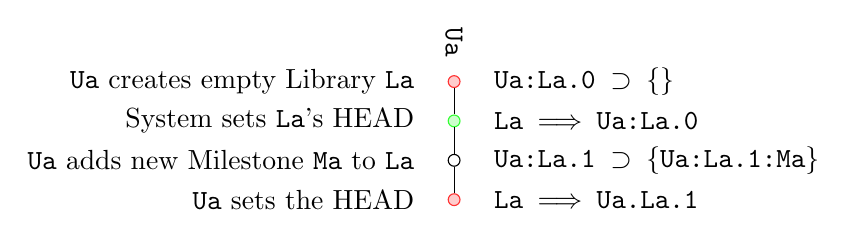
\begin{tikzpicture}[
				save/.style={circle,draw,minimum size=1.5mm},
				branch/.style={circle,draw=red!80,fill=red!20,minimum size=1.5mm},
				heads/.style={circle,draw=green!80,fill=green!20,minimum size=1.5mm},
				branchfrom/.style={circle},
				labr/.style={anchor=west,font=\tt},
				labl/.style={anchor=east},
				bend angle=45,
				inner sep=0pt]
				\node at (0,5mm) [rotate=270] {\Ua};
				\node [branch] 		(UaLa0) 		at (0,0)				{};
					\node [labr] at (5mm,0) 	{Ua:La.0 \eq \{\}};
					\node [labl] at (-5mm,0)	{\Ua\ creates empty Library \La};
				\node [heads]		(LaUaLa0)		at (0,-5mm)			{}
					edge [-] (UaLa0);
					\node [labr] at (5mm,-5mm)	{La \hto Ua:La.0};
					\node [labl] at (-5mm,-5mm)	{System sets \La's HEAD};
				\node [save]		(UaLa1)		at (0,-10mm)			{}
					edge [-] (LaUaLa0); 
					\node [labr] at (5mm,-10mm)	{Ua:La.1 \eq \{Ua:La.1:Ma\}};
					\node [labl] at (-5mm,-10mm)	{\Ua\ adds new Milestone \Ma\ to \La};
				\node [branch]		(LaUaLa1)		at (0,-15mm)			{}
					edge [-] (UaLa1);
					\node [labr] at (5mm,-15mm) 	{La \hto Ua.La.1};
					\node [labl] at (-5mm,-15mm)	{\Ua\ sets the HEAD};
			\end{tikzpicture}
			
	\subsection{Scenario (1 Module, 2 Users, no dependencies)}
		\Ua\ and \Ub\ are working on \La\\
		\Ub\ modified one module

		\vspace{5mm}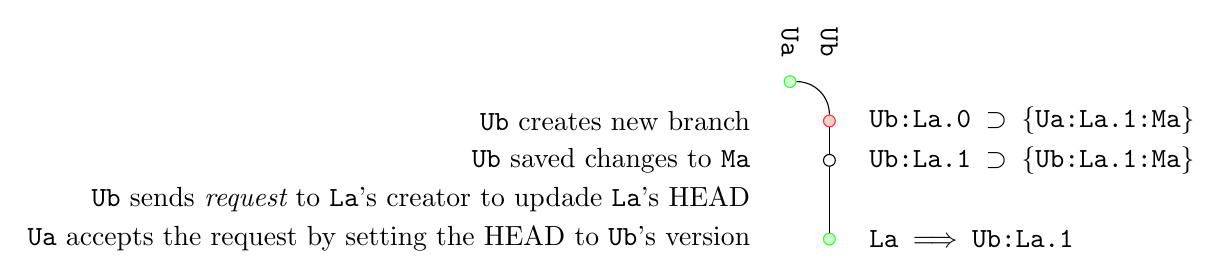
\begin{tikzpicture}[
			save/.style={circle,draw,minimum size=1.5mm},
			branch/.style={circle,draw=red!80,fill=red!20,minimum size=1.5mm},
			heads/.style={circle,draw=green!80,fill=green!20,minimum size=1.5mm},
			branchfrom/.style={circle},
			labr/.style={anchor=west,font=\tt},
			labl/.style={anchor=east},
			bend angle=45,
			inner sep=0pt]
			\node at (0,5mm) [rotate=270] {\Ua};\node at (5mm,5mm) [rotate=270] {\Ub};
			\node [heads] 		(UaLa1) 		at (0,0)				{};
			\node [branch]		(UbLa0)		at (5mm,-5mm)			{}
				edge [-,bend right] (UaLa1); 
				\node [labr] at (10mm,-5mm)	{Ub:La.0 \eq \{Ua:La.1:Ma\}};
				\node [labl] at (-5mm,-5mm)	{\Ub\ creates new branch};
			\node [save]		(UbLa1)		at (5mm,-10mm)			{}
				edge [-] (UbLa0);
				\node [labr] at (10mm,-10mm)	{Ub:La.1 \eq \{Ub:La.1:Ma\}};
				\node [labl] at (-5mm,-10mm)	{\Ub\ saved changes to \Ma};
				\node [labl] at (-5mm,-15mm)	{\Ub\ sends {\em request} to \La's creator to updade \La's HEAD};
			\node [heads]		(LaUbLa1)		at (5mm,-20mm)			{}
				edge[-] (UbLa1);
				\node [labr] at (10mm,-20mm)	{La \hto Ub:La.1};
				\node [labl] at (-5mm,-20mm)	{\Ua\ accepts the request by setting the HEAD to \Ub's version};
		\end{tikzpicture}\vspace{5mm}

		\noindent Result: {\tt La \hto  Ub:La.1 \eq \{Ub:La.1:Ma\}}

	\subsection{Scenario (2 Modules, 2 Users, no dependencies)}

		\Ua\ and \Ub\ are working on \La\\ 
		\Ua\ created module \Mb\\
		\Ub\ is working on \Mb\
		
		\vspace{-3mm}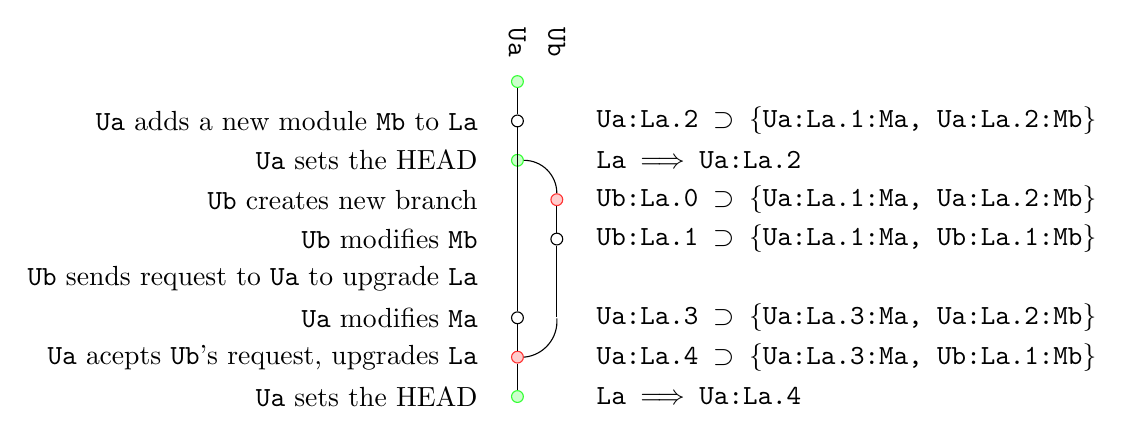
\begin{tikzpicture}[
			save/.style={circle,draw,minimum size=1.5mm},
			branch/.style={circle,draw=red!80,fill=red!20,minimum size=1.5mm},
			heads/.style={circle,draw=green!80,fill=green!20,minimum size=1.5mm},
			branchfrom/.style={circle},
			point/.style={circle,minimum size=0pt},
			labr/.style={anchor=west,font=\tt},
			labl/.style={anchor=east},
			bend angle=45,
			inner sep=0pt]
			\node at (0,5mm) [rotate=270] {\Ua};\node at (5mm,5mm) [rotate=270] {\Ub};
			\node [heads] 		(UaLa1) 		at (0,0)					{};
			\node [save]			(UaLa2)		at (0,-5mm)				{}
				edge [-] (UaLa1);
				\node [labr] at (10mm,-5mm)	{Ua:La.2 \eq \{Ua:La.1:Ma, Ua:La.2:Mb\}};
				\node [labl] at (-5mm,-5mm)	{\Ua\ adds a new module \Mb\ to \La};
			\node [heads]			(LaUaLa2)		at (0,-10mm)				{}
				edge [-] (UaLa2);
				\node [labr] at (10mm,-10mm) {La \hto Ua:La.2};
				\node [labl] at (-5mm,-10mm) {\Ua\ sets the HEAD};
			\node [branch]		(UbLa0)		at (5mm,-15mm)			{}
				edge [-,bend right] (LaUaLa2);
				\node [labr] at (10mm,-15mm) {Ub:La.0 \eq \{Ua:La.1:Ma, Ua:La.2:Mb\}};
				\node [labl] at (-5mm,-15mm) {\Ub\ creates new branch};
			\node [save] 			(UbLa1)		at (5mm,-20mm)			{}
				edge [-] (UbLa0);
				\node [labr] at (10mm,-20mm) {Ub:La.1 \eq \{Ua:La.1:Ma, Ub:La.1:Mb\}};
				\node [labl] at (-5mm,-20mm) {\Ub\ modifies \Mb};
				\node [labl] at (-5mm,-25mm) {\Ub\ sends request to \Ua\ to upgrade \La};
				\node [point] (p1) at (5mm,-30mm) {} edge [-] (UbLa1);
			\node [save]			(UaLa3)		at (0,-30mm)				{}
				edge [-] (UaLa2);
				\node [labr] at (10mm,-30mm) {Ua:La.3 \eq \{Ua:La.3:Ma, Ua:La.2:Mb\}};
				\node [labl] at (-5mm,-30mm) {\Ua\ modifies \Ma};
			\node [branch]		(UaLa4)		at (0,-35mm)				{}
				edge [-] (UaLa3)
				edge [-,bend right] (p1);
				\node [labr] at (10mm,-35mm) {Ua:La.4 \eq \{Ua:La.3:Ma, Ub:La.1:Mb\}};
				\node [labl] at (-5mm,-35mm) {\Ua\ acepts \Ub's request, upgrades \La};
			\node [heads]			(LaUaLa4)		at (0,-40mm)				{}
				edge [-] (UaLa4);
				\node [labr] at (10mm,-40mm) {La \hto Ua:La.4};
				\node [labl] at (-5mm,-40mm) {\Ua\ sets the HEAD};
		\end{tikzpicture}\vspace{4mm}

		\noindent Result: {\tt La \hto Ua:La.4 \eq \{Ua:La.3:Ma, Ub:La.1:Mb\}}

	\subsection{Scenario (2 Modules, 2 Users, no dependencies)}
	
		\Ua\ and \Ub\ are working on \La\\ 
		\Ub\ created module \Mb\
		
		\begin{enumerate}
			\item{\Ub\ adds a new module \Mb\ to \La\\
				{\tt Ub:La.0 \eq \{Ua:La.1:Ma\}} --- automatic fork of \La\\
				{\tt Ub:La.1 \eq \{Ua:La.1:Ma, Ua:La.1:Mb\}}
			}
			\item{\Ub\ modifies \Mb\\
				{\tt Ub:La.2 \eq \{Ua:La.1:Ma, Ub:La.2:Mb\}}
			}
			\item{\Ub\ sends request to \Ua\ to upgrade \La\ from {\tt Ub:La.2}}
			\item{\Ua\ modifies \Ma\\
				{\tt Ua:La.2 \eq \{Ua:La.2:Ma\}}
			}
			\item{\Ua\ acepts \Ub's request\\
				{\tt Ua:La.3 \eq \{Ua:La.2:Ma, Ub:La.2:Mb\}}
			}
			\item{\Ua\ sets the HEAD\\
				{\tt La \hto Ua:La.3}
			}
			\item{Result: {\tt La \hto Ua:La.3 \eq \{Ua:La.2:Ma, Ub:La.2:Mb\}}}
		\end{enumerate}

	\subsection{Scenario with conflict (2 Modules, 2 Users, no dependencies)}

		\Ua\ and \Ub\ are working on \La\\ 
		\Ua\ created module \Mb\\
		\Ua\ and \Ub\ are working on \Mb\\
		Conflict arises...

		\begin{enumerate}
			\item{\Ua\ adds a new module \Mb\ to \La\\
            		{\tt Ua:La.2 \eq \{Ua:La.1:Ma, Ua:La.2:Mb\}}
			}
			\item{\Ua\ sets the HEAD\\
				{\tt La \hto Ua:La.2}
			}
			\item{\Ub\ modifies \Mb\\
				{\tt Ub:La.0 \eq \{Ua:La.1:Ma, Ua:La.2:Mb\}} --- automatic fork of \La\\
				{\tt Ub:La.1 \eq \{Ua:La.1:Ma, Ub:La.1:Mb\}}
			}
			\item{\Ua\ modifies \Mb\\
				{\tt Ua:La.3 \eq \{Ua:La.1:Ma, Ua:La.2:Mb\}}
			}
			\item{{\bf CONFLICT}\\
            		At the time we've got two versions of La.Mb which came out from the same version
            	}
            	\item{\Ua\ sets the HEAD\\
            		{\tt La \eq Ua:La.3}
            	}
            	\item{\Ub\ receives info that his source is behind the HEAD\\
				{\tt Ub:La.1:Mb} (and {\tt Ub:La.1}) is marked as {\em conflicted}\\
				\Ub\ can't send the update request
			}
			\item{\Ub\ manually solves conflict by editing the \Mb\ and removing the {\em conflict flag}\\
				{\tt Ub:La.2 \eq \{Ua:La.1, Ub:La.2:Mb\}}
			}
			\item{\Ub\ sends request to \Ua\ to upgrade \La\ from {\tt Ub:La.2}}
			\item{\Ua\ acepts \Ub's request\\
				{\tt Ua:La.4 \eq \{Ua:La.3:Ma, Ub:La.2:Mb\}}
			}
			\item{\Ua\ sets the HEAD\\
				{\tt La \hto Ua:La.4}
			}
			\item{Result: {\tt La \hto Ua:La.4 \eq \{Ua:La.3:Ma, Ub:La.2:Mb\}}}
		\end{enumerate}
		
	\subsection*{Draft/Ideas}
	\begin{description}
		\item[update Library] if Library HEAD has been changed something should tell the User that an update is possible. It should then (on request) change the versions of all Modules which are not in conflict with updating Library. In essence, if \\
			{\tt Ua:La.1 \eq \{Ua:La.1:Ma, Ub:La.2:Mb\}} is a Library to be updated and \\
			{\tt La \hto Uc:La.3 \eq \{Ub:La.1:Ma, Uc:La.3:Mb, Uc:La.1:Mc\}} is current HEAD, then\\
			{\tt Ub:La.2:Mb} should be updated to {\tt Uc:La.3:Mb} and {\tt Uc:La.1:Mc} should be added.\\
			User should receive a notification that {\tt Ua:La.1:Ma} is not in sync with HEAD.
		\item[forking] Consider forcing users to create their copy of a Package before entering to edit mode (as in {\em github}), find a better name if needed ...
		\item[revision graphs] should be created inside this documentation. \\
			Consider using tikz \url{http://www.texample.net/tikz/examples/}
	\end{description}

	\subsection*{To be continued\ldots}
\end{document}
